\documentclass[10pt,letterpaper]{article}

\usepackage{hyperref}
\usepackage{cogsci}
\usepackage{pslatex}
\usepackage{apacite}
\usepackage{graphicx}
\usepackage{todonotes}

\title{Extremely costly intensifiers are stronger than quite costly ones.}
 
\author{{\large \bf Erin Bennett (erindb@stanford.edu)} \\
  Department of Psychology, 450 Serra Mall , Stanford, CA 94305
  \AND {\large \bf Noah Goodman (ngoodman@stanford.edu)} \\
  Department of Psychology, 450 Serra Mall , Stanford, CA 94305}


\begin{document}

\maketitle


\begin{abstract}
%Intensifiers of scalar adjectives might derive the degree of their meaning from their cost.
%We show that surprisal and syllable length, two different construals of the cost of an intensifier, both independently predict estimates of degree.
%We further show that when an intensifier is frequently repeated within a ``non-standard dialect of English'' (i.e. when we manipulate the surprisal of an intensifier), its inferred degree is consequently lower.

\todo[inline]{abstract}

\textbf{Keywords:} 
intensifiers; degree adverbs; scalar adjectives; pragmatics; m-implicature
\end{abstract}


\section{Introduction}

\todo[inline]{complexity, bouba/kiki, m-implicature, ...}

%Intensifiers, for example ``extremely'' or ``very'', are adverbs that modify scalar adjectives to increase the degree.
%These words are numerous in English, are relatively easy to coin, and the use of one intensifier over another (e.g. ``wicked fun'' rather than ``totally fun'') often suggests membership in a particular social group or dialect.

%We provide evidence for the claim that intensifiers' meanings are derived from pragmatic inference. The cost of uttering an intensifier, which we approximate using syllable length and also surprisals calculated from corpus frequencies from Google Ngrams, largely predicts the degree people will ascribe to it.
%When we create an imaginary dialect of English in which a particular intensifier is overused, we find that that intensifier is inferred to have a weeker meaning than when it is not repeated.

%Scalar adjectives, free semantic threshold variables, and m-implicature. Language change.

% To explore the hypothesis that the meanings of intensifiers are a function of their cost, we first wanted to see whether surprisal and syllable length (two different ways of measuring the cost of a word) were even correlated with the meanings of intensifiers. We ran two experiments: one with a free response dependent measure and one with a ranking dependent measure.

\section{Experiment 1}

To explore the hypothesis that the meanings of intensifiers are a function of their cost, we first wanted to see whether two possible ways of measuring the cost of a word, surprisal and syllable length, were correlated with the meanings of intensifiers.

\subsection{Method\footnote{The full experiment can be found at \url{http://web.stanford.edu/~erindb/degree-adverbs/experiments/exp5_2014-12-01/exp5.html}}}

40 participants with US IP addresses participated in our Experiment 1 on Amazon's Mechanical Turk.

In Expeirment 1, we used a free response dependent measure to elicit prices in dollars of objects (coffee makers, watches, and laptops) that were described as ``\emph{[intensifier]} expensive'' (Fig~\ref{exp1-q}). We required that participants gave their price as an integer number of dollars or as a number with two digits after the decimal point. We included 40 intensifiers in this experiment (Table~\ref{exp1-intensifiers}). Both objects and intensifiers were varied exhaustively within participants.

To calculate the surprisal of an intensifier, we approximated the probability by the proportion of occurances in the Google Web 1T 5-grams database \cite{web1t5gram}
\footnote{
We also ran the same analyses on frequency information collected from the Google Books American Ngrams Corpus \cite{books2011} as well, and found similar results.

In addition, we did the same using the bigram frequencies of ``\emph{[intensifer]} expensive'' rather than the unigram frequencies of the intensifiers alone. These data were much more sparse. For bigrams, we found no significant effects of surprisal using the books database and a negative effect using the web database.
}


% We ran the same analysis using surprisal calculated in different ways from different sources. Our results were similar for unigrams taken from 
% We also ran our analysis calculating surprisal based on bigrams  corpus and using both unigrams and bigrams from the Google Books database.}\todo{need to rerun with web bigrams (results are different, data is sparse), books unigrams, and books bigrams.}.

If the meaning of an intensifier is stronger for higher cost intensifiers, we would expect to find that as surprisal and length in syllables increase, the prices participants give will also increase.

\begin{figure}[ht]
\begin{center}
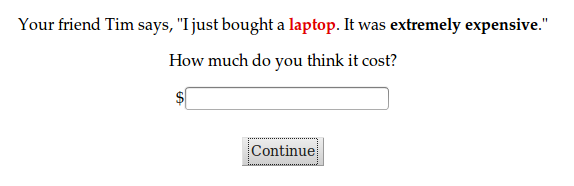
\includegraphics[width=0.4\textwidth]{analysis_files/images/exp1-q.png}
\end{center}
\caption{Screenshot from Experiment 1 target question.} 
\label{exp1-q}
\end{figure}

\subsection{Results}

We find that participants' price responses increase as both surprisal and length in syllables increase (Fig~\ref{exp1-plot}).

\begin{figure}[ht]
\begin{center}
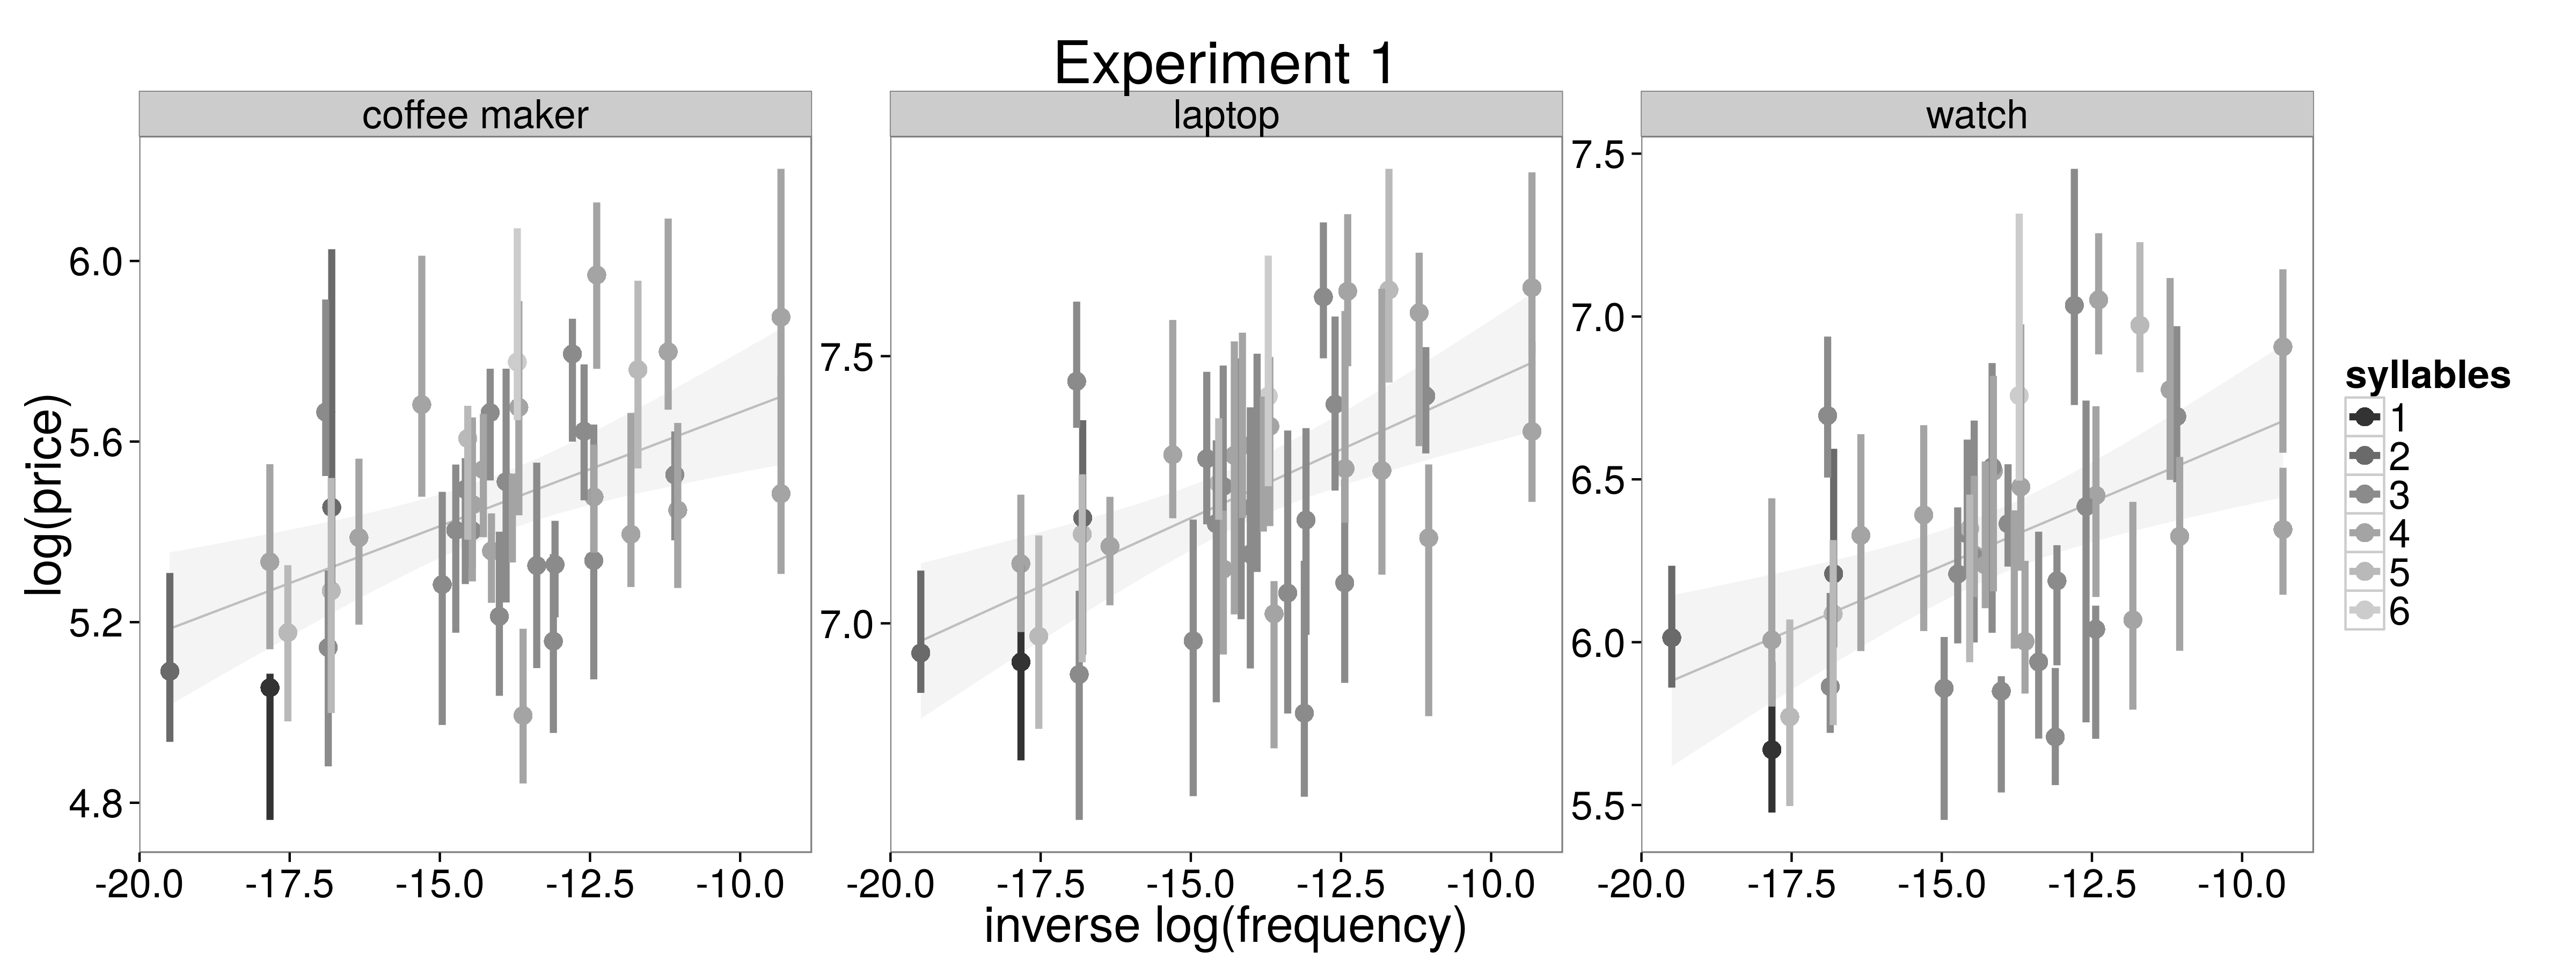
\includegraphics[width=0.48\textwidth]{analysis_files/images/exp1-plot.png}
\end{center}
\caption{Results of Experiment 1. As surprisal and length in syllables increase, participants' free response prices increased.} 
\label{exp1-plot}
\end{figure}

In a linear mixed effects regression with syllables and surprisal and their interaction as fixed effects\footnote{We centered both surprisal and syllable length by subtracting their means.} and random intercepts and slopes for syllables and surprisal for both participant and object, we found significant main effects of surprisal (estimate=0.054, p=0.012) and syllable length  (estimate=0.093, p=0.0041) as well as a significant interaction (estimate=0.019, p=0.00018).
%anything more complicated won't converge

\subsection{Discussion}

We found that both our measures of cost (surprisal and syllable length) predict participants' estimates of price.
This suggests that intensifiers that are more surprising and longer (and therefore are more costly to utter) also have stronger meanings.

The relationship between strength and suprisal could be explained by the stronger meanings themselves being more unusual and surprising and therefore corresponding to words that are used less frequently.
However, this story would not be able to explain why syllable length above and beyond surprisal would predict stronger meanings.

\section{Experiment 2}

In Experiment 2, we replicated our finding from Experiment 1 using a slightly different dependent measure: rankings.

\subsection{Method\footnote{The full experiment can be found at \url{http://web.stanford.edu/~erindb/degree-adverbs/experiments/exp4/exp4.html}}}

We divided the 40 intensifiers from Experiment 1 into four lists (Table~\ref{exp2-intensifiers}). We asked 30 participants with US IP addresses on Amazon Mechanical Turk to order (by draggging and dropping) four sets of 10 adjective phrases from most to least strong (Fig~\ref{exp2-q}). Each set of adjective phrases repeated the same adjective (``old'', ``expensive'', ``beautiful'', or ``tall'') paired with the intensifiers from one of the intensifier lists. The pairings between the four intensifier lists and the four adjectives were randomized between participants.

\begin{figure}[ht]
\begin{center}
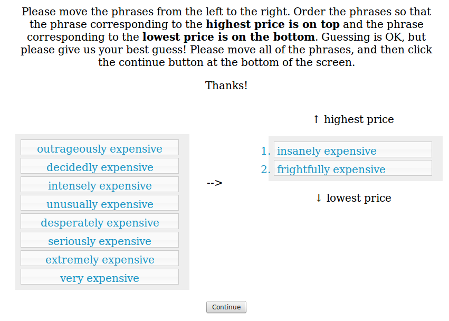
\includegraphics[width=0.4\textwidth]{analysis_files/images/exp2-q.png}
\end{center}
\caption{Screenshot from Experiment 2 target question.} 
\label{exp2-q}
\end{figure}

\subsection{Results}

In a linear regression of ranking within the list as a function of surprisal, syllable length, and their interaction\footnote{We centered both surprisal and syllable length by subtracting their means.}, we found significant main effects of surprisal (estimate=0.46, p$<$2e-16) and syllables (estimate=0.64, p=8.2e-11) as well as a significant interaction (estimate=0.069, p=0.046).

\begin{figure}[ht]
\begin{center}

\includegraphics[width=0.48\textwidth]{analysis_files/images/exp2-plot.png}
\end{center}
\caption{Results of Experiment 2. As surprisal and length in syllables increase, participants' rankings increased.} 
\label{exp2-plot}
\end{figure}

\subsection{Discussion}

We again found that participants assign stronger meanings to intensifiers with higher surprisals and syllable lengths.

\section{Experiment 3}

In Experiment 3, we tested whether manipulating the surprisal associated with an intensifier can change the strength of an intensifier. If this were the case, it would provide more evidence for our hypothesis that the surprisal of a word causes its meaning to be stronger due to the added cost.

\subsection{Method\footnote{The full experiment can be found at \url{http://web.stanford.edu/~erindb/degree-adverbs/experiments/exp8/exp8.html}}}

We looked at two short intensifiers of equal length: ``truly'' and ``very''. In our two conditions (varied between participants), each intensifier was either the target or the control. In a comic-style training story, the target intensifier was repeated 22 times by a speaker who lived ``across the country'' and had ``a distinct way of speaking.'' The control intensifier was not used by the speaker in the story.

To guage whether participants had learned that the speaker's use of the target intensifier was unusually high, we asked participants how many times in the next 1000 words they thought the speaker would use the control word, the target word, and another word that had been frequently repeated.

To determine what strength participants inferred for the target and control intensifiers, we gave participants a final panel of the comic where the speaker described a new coffee maker he bought (Fig~\ref{exp3-q}). We asked participants to guess the price of the coffee maker given different possible descriptions the speaker could have used.

\begin{figure}[ht]
\begin{center}
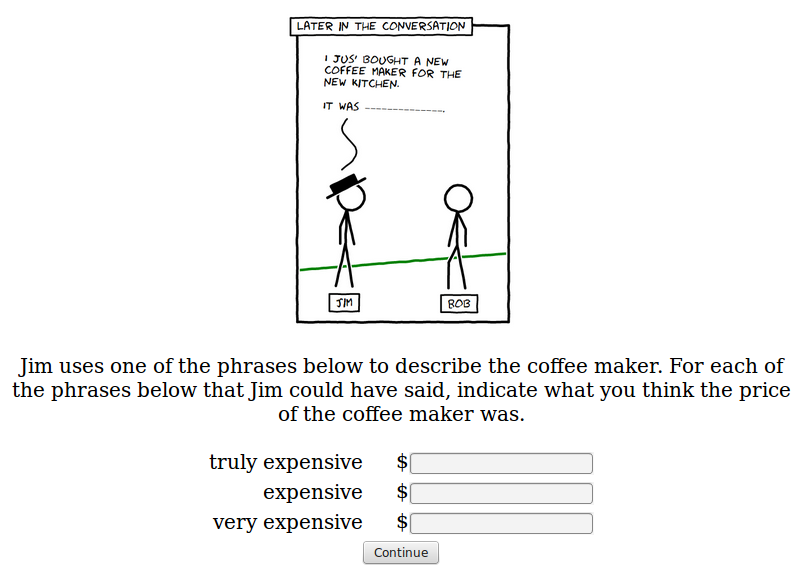
\includegraphics[width=0.4\textwidth]{analysis_files/images/exp3-q.png}
\end{center}
\caption{Screenshot from Experiment 3 target question.} 
\label{exp3-q}
\end{figure}

\subsection{Results}

We found that participants did learn that the speaker's use of a word was much higher when it was a target than when it was a control (Fig~\ref{exp3-freq-plot}). In a linear regression with word type (target or control) as a fixed effect and random intercepts for word and participant, word type was a significant predictor of frequency (estimate=34.06, p=0.0405).

In addition, when participants believed the speaker's use of a word was much higher, they believed the meaning the speaker intended to convey with the word was lower (Fig~\ref{exp3-price-plot}). The difference between ``\emph{(truly|very)} expensive'' and ``expensive'' was greater for the target word than for the control word. In a linear gregression with word type as a fixed effect and random intercepts for word and participant, word type was a significant predictor of difference score (estimate=-31.39, p=0.0226).

In a linear regression with word type (target or control) as a fixed effect and random intercepts for word and participant, word type was a significant predictor of frequency (estimate=34.06, p=0.0405).

Individuals' estimates of frequency correlate with their estimates of price (Fig~\ref{exp3-scatterplot}, Pearson's r=0.396, p=0.0169).

\begin{figure}[ht]
\begin{center}
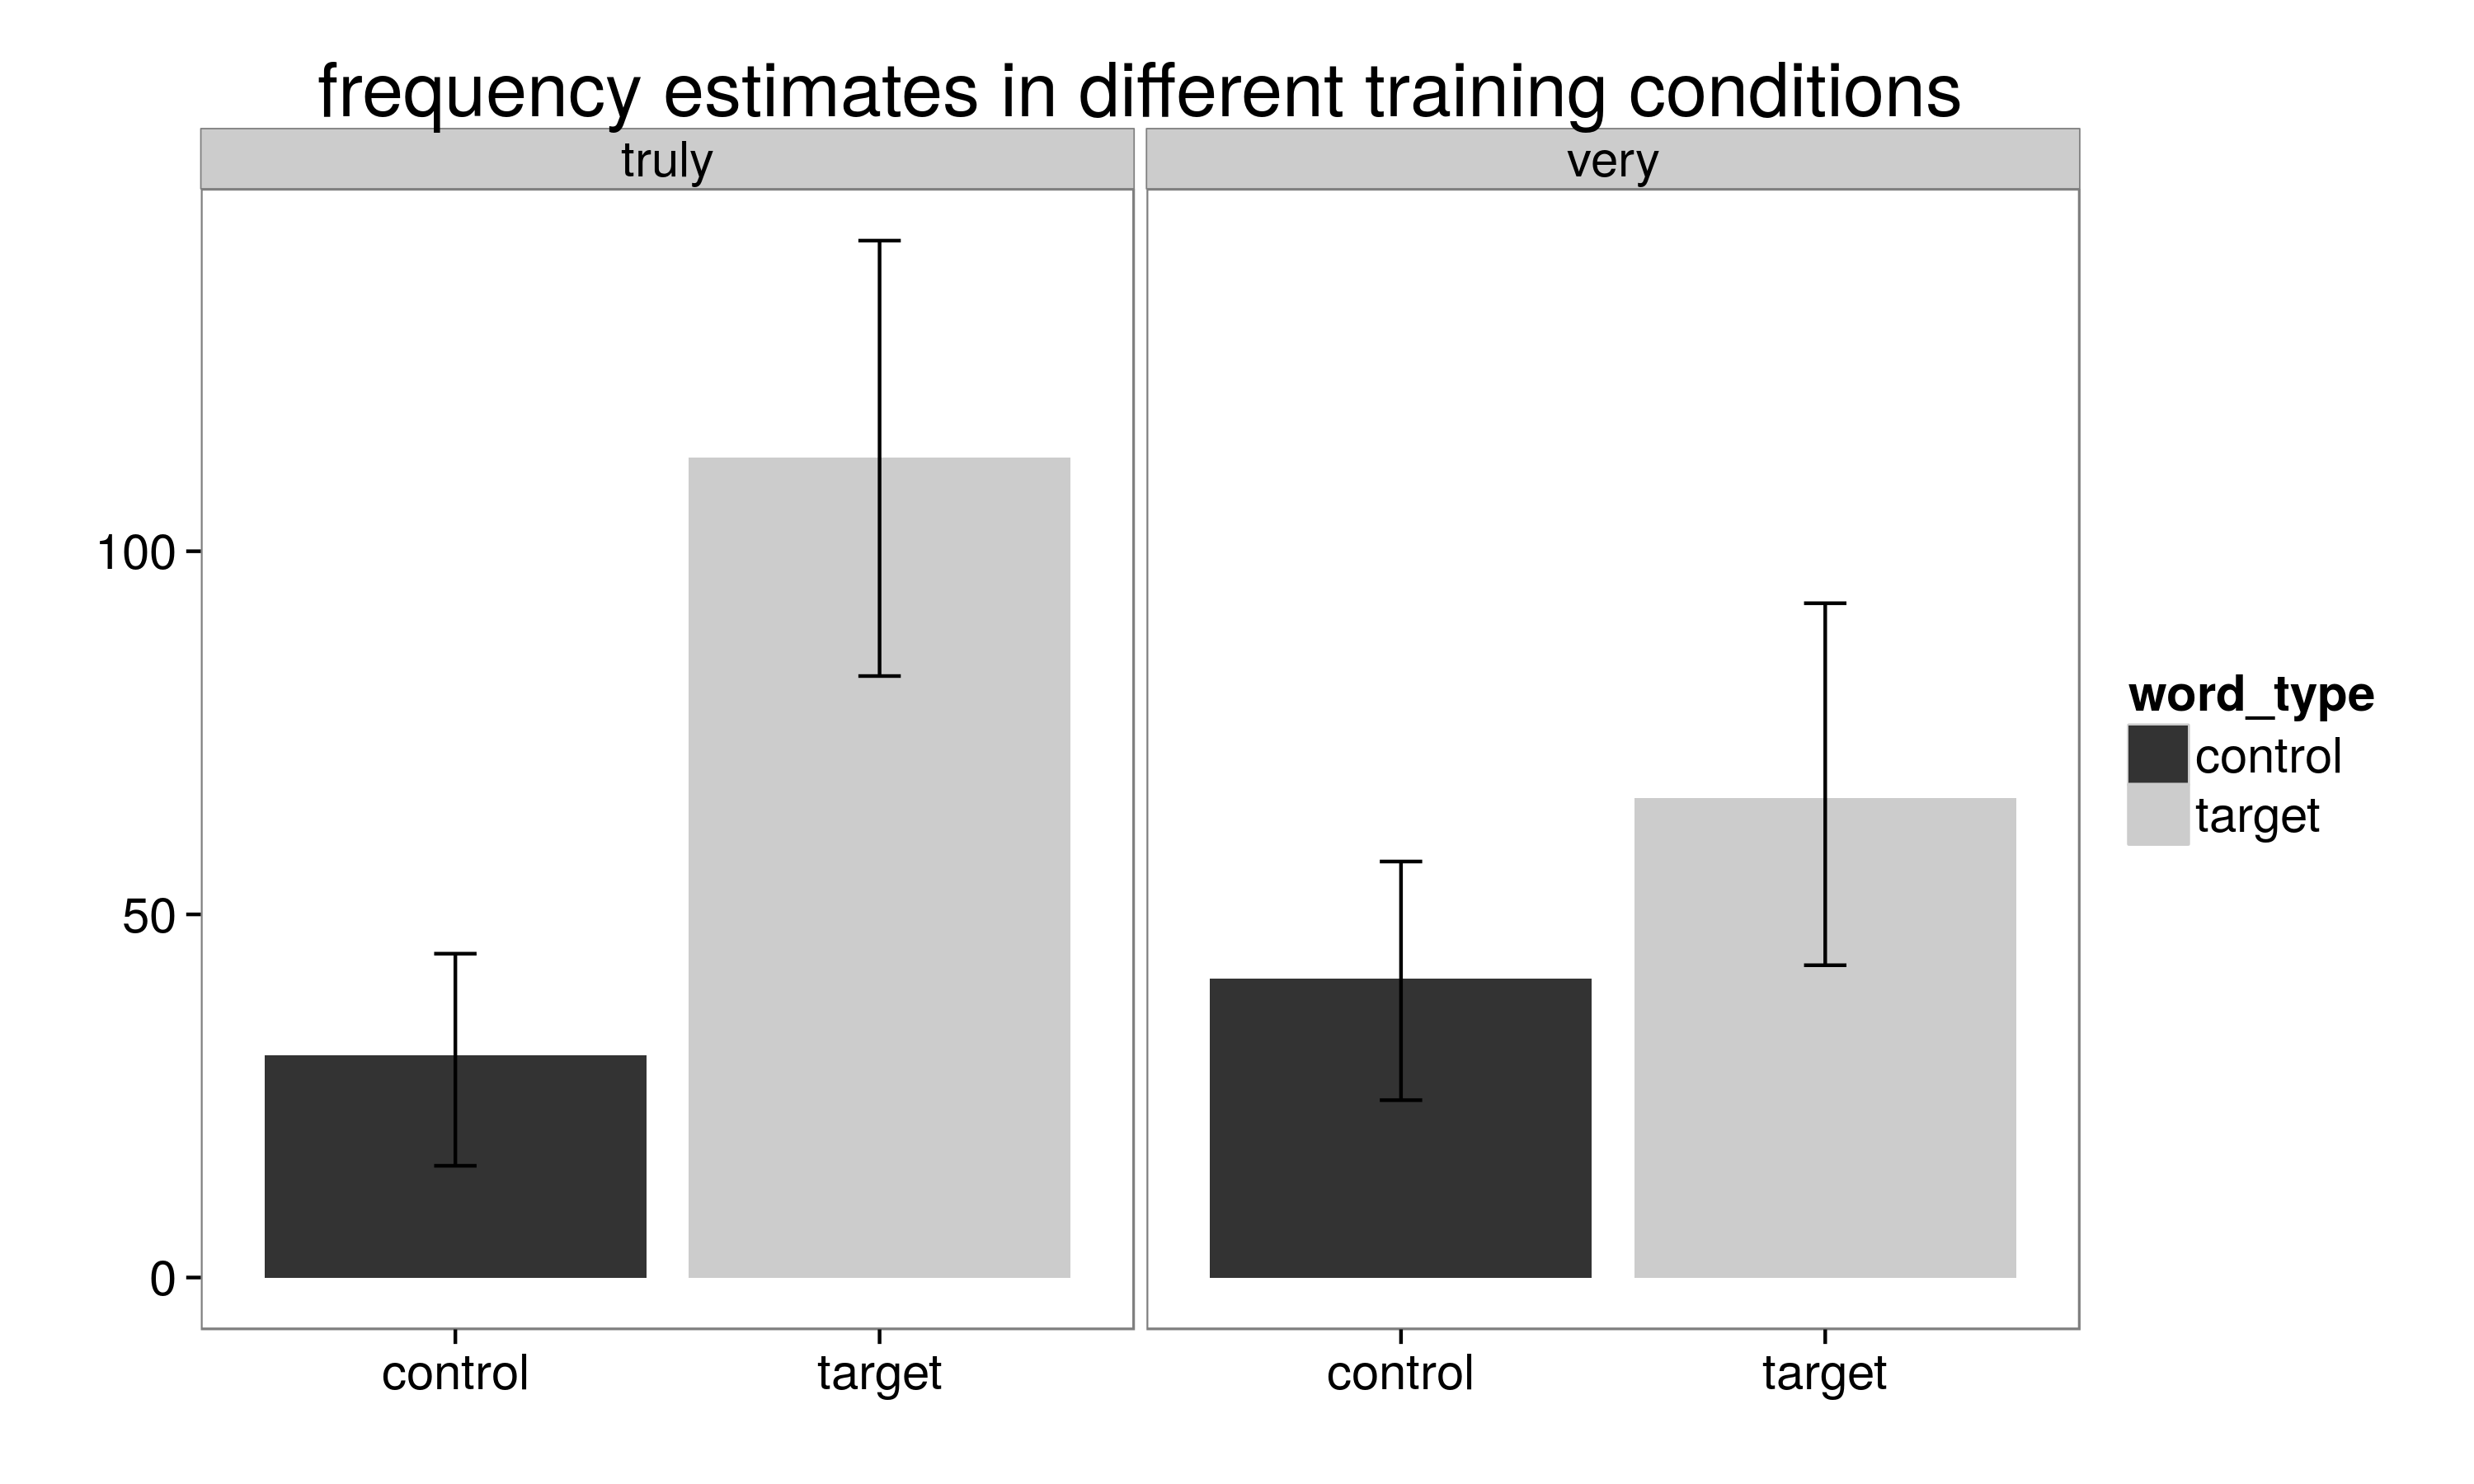
\includegraphics[width=0.48\textwidth]{analysis_files/images/exp3-freq-plot}
\end{center}
\caption{Results of Experiment 3. Intensifier is given a higher frequency estimate when it is target than when it is control, showing that participants learned a new frequency for that intensifier from the training.} 
\label{exp3-freq-plot}
\end{figure}

\begin{figure}[ht]
\begin{center}
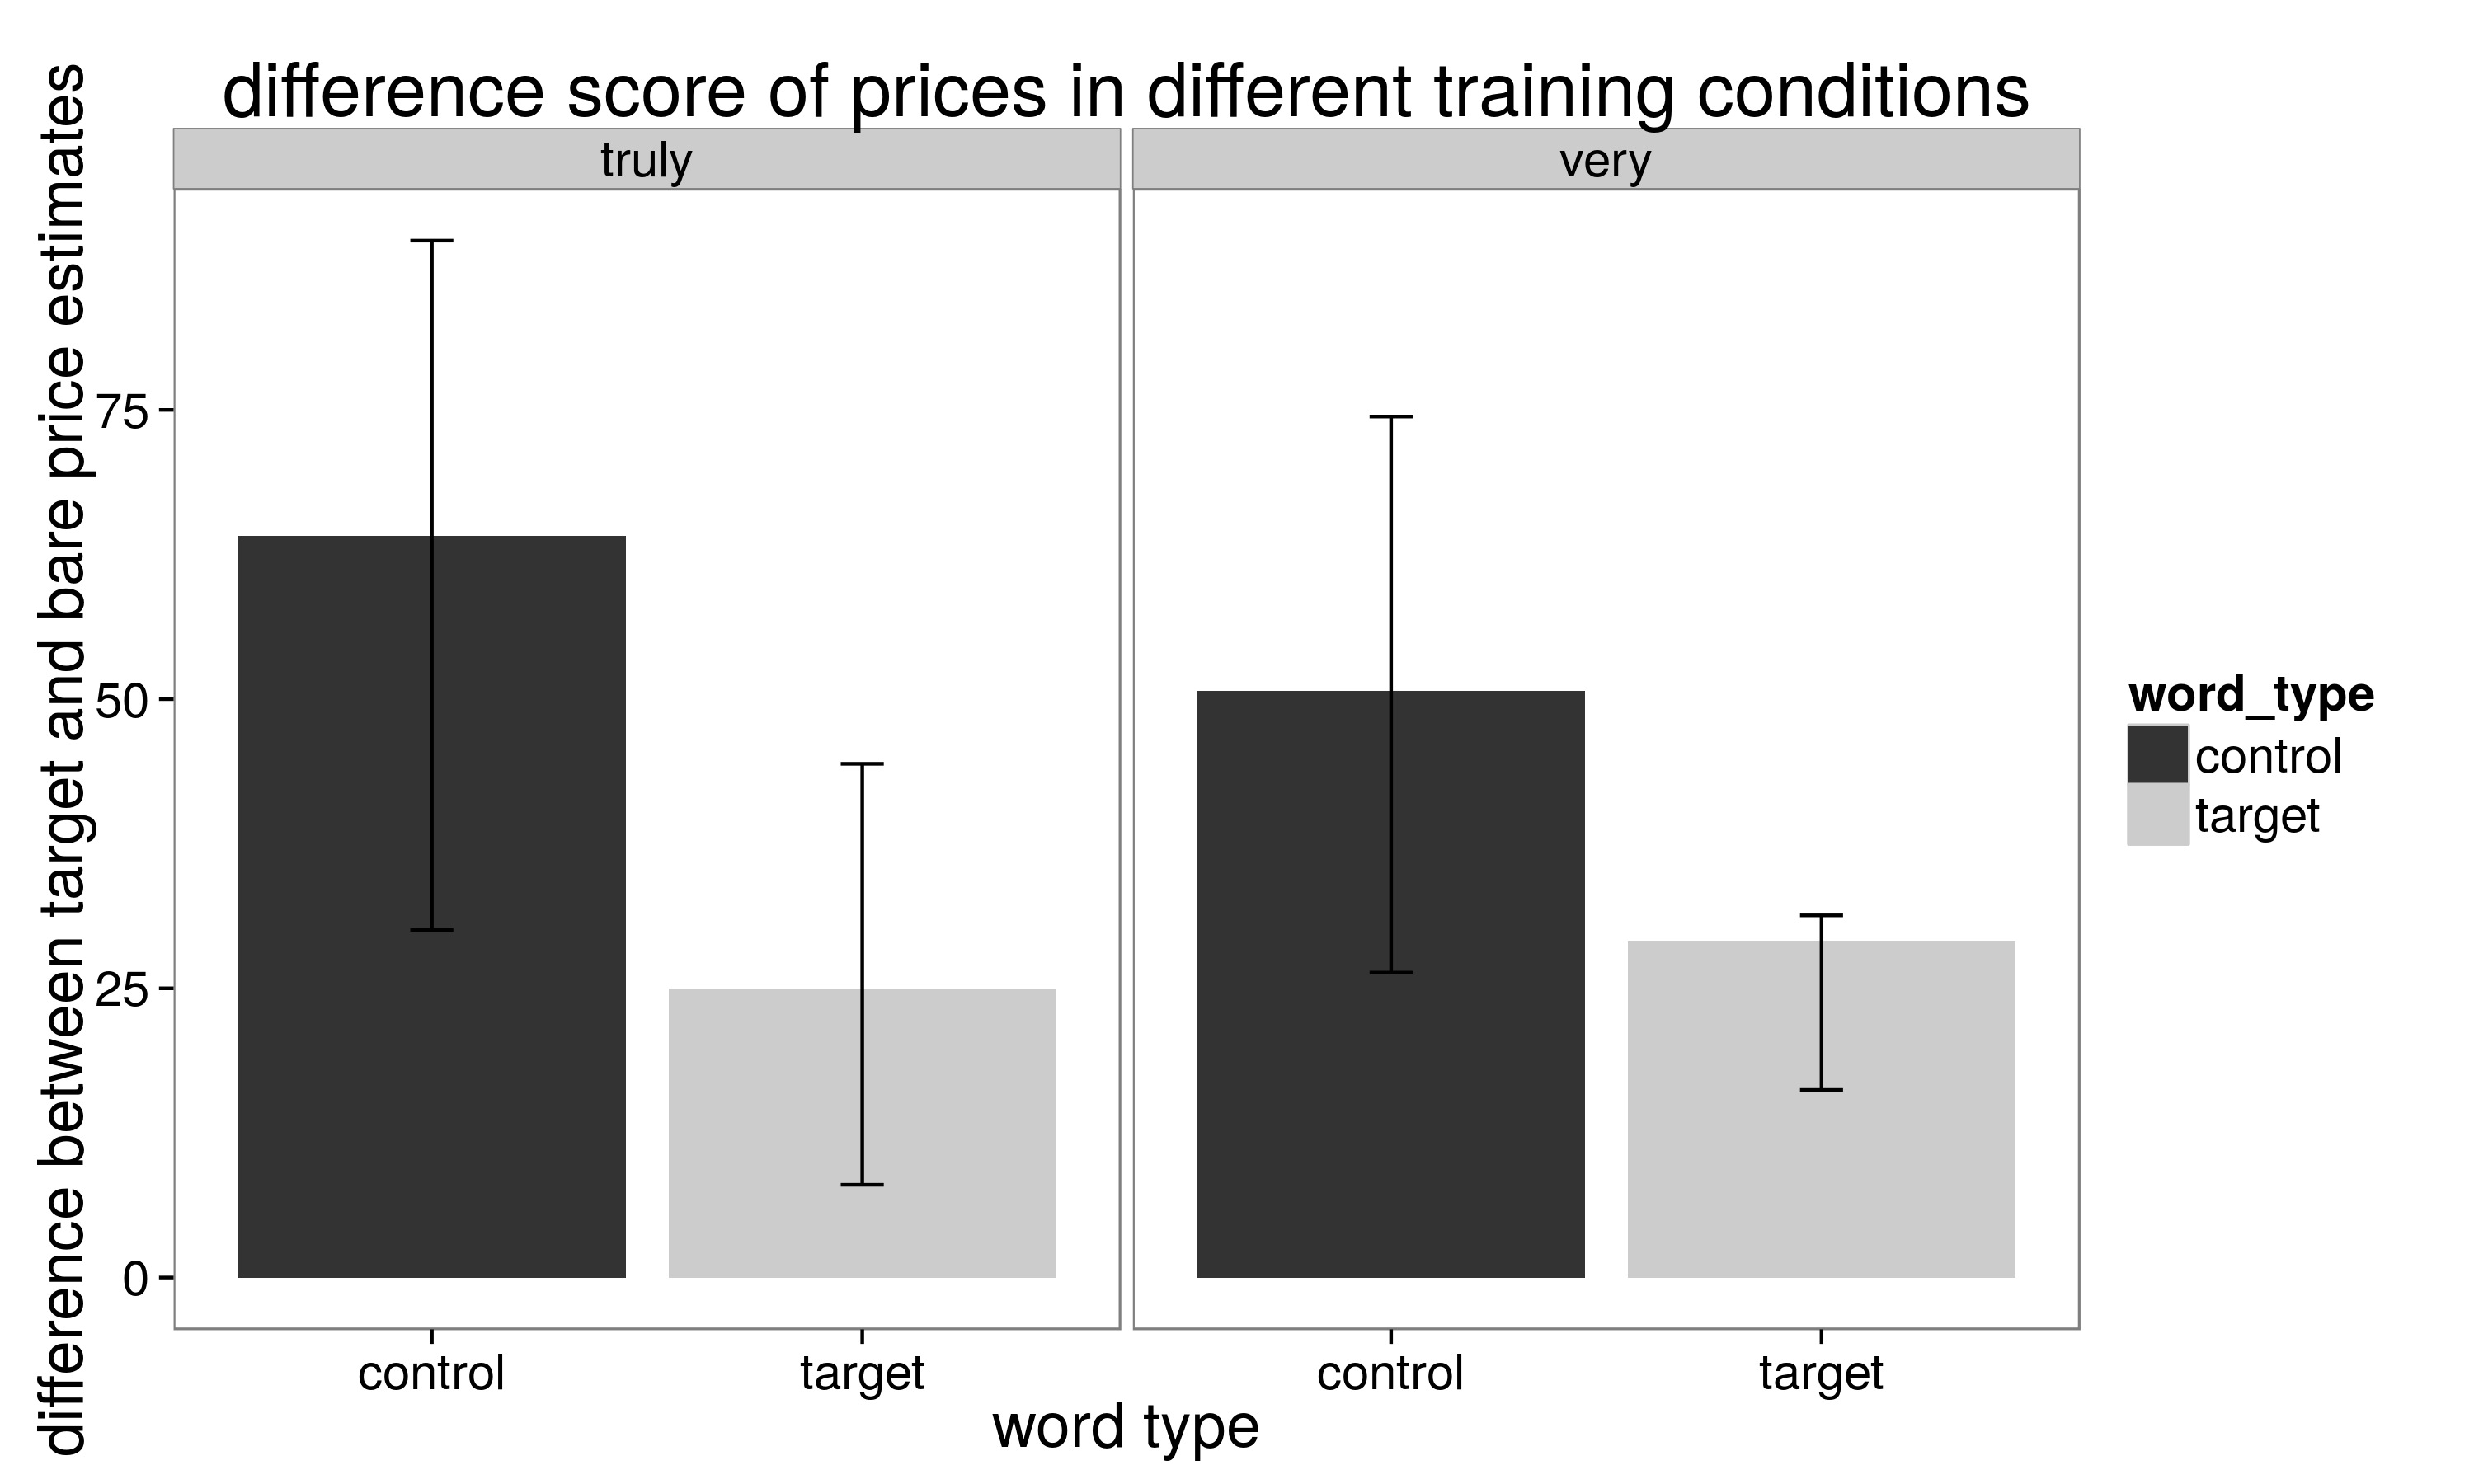
\includegraphics[width=0.48\textwidth]{analysis_files/images/exp3-price-plot.png}
\end{center}
\caption{Results of Experiment 3. Price estimate for intensifier is lower after the intensifier is repeated (target condition), showing that overuse within a dialect results in a less strong meaning.} 
\label{exp3-price-plot}
\end{figure}

\begin{figure}[ht]
\begin{center}
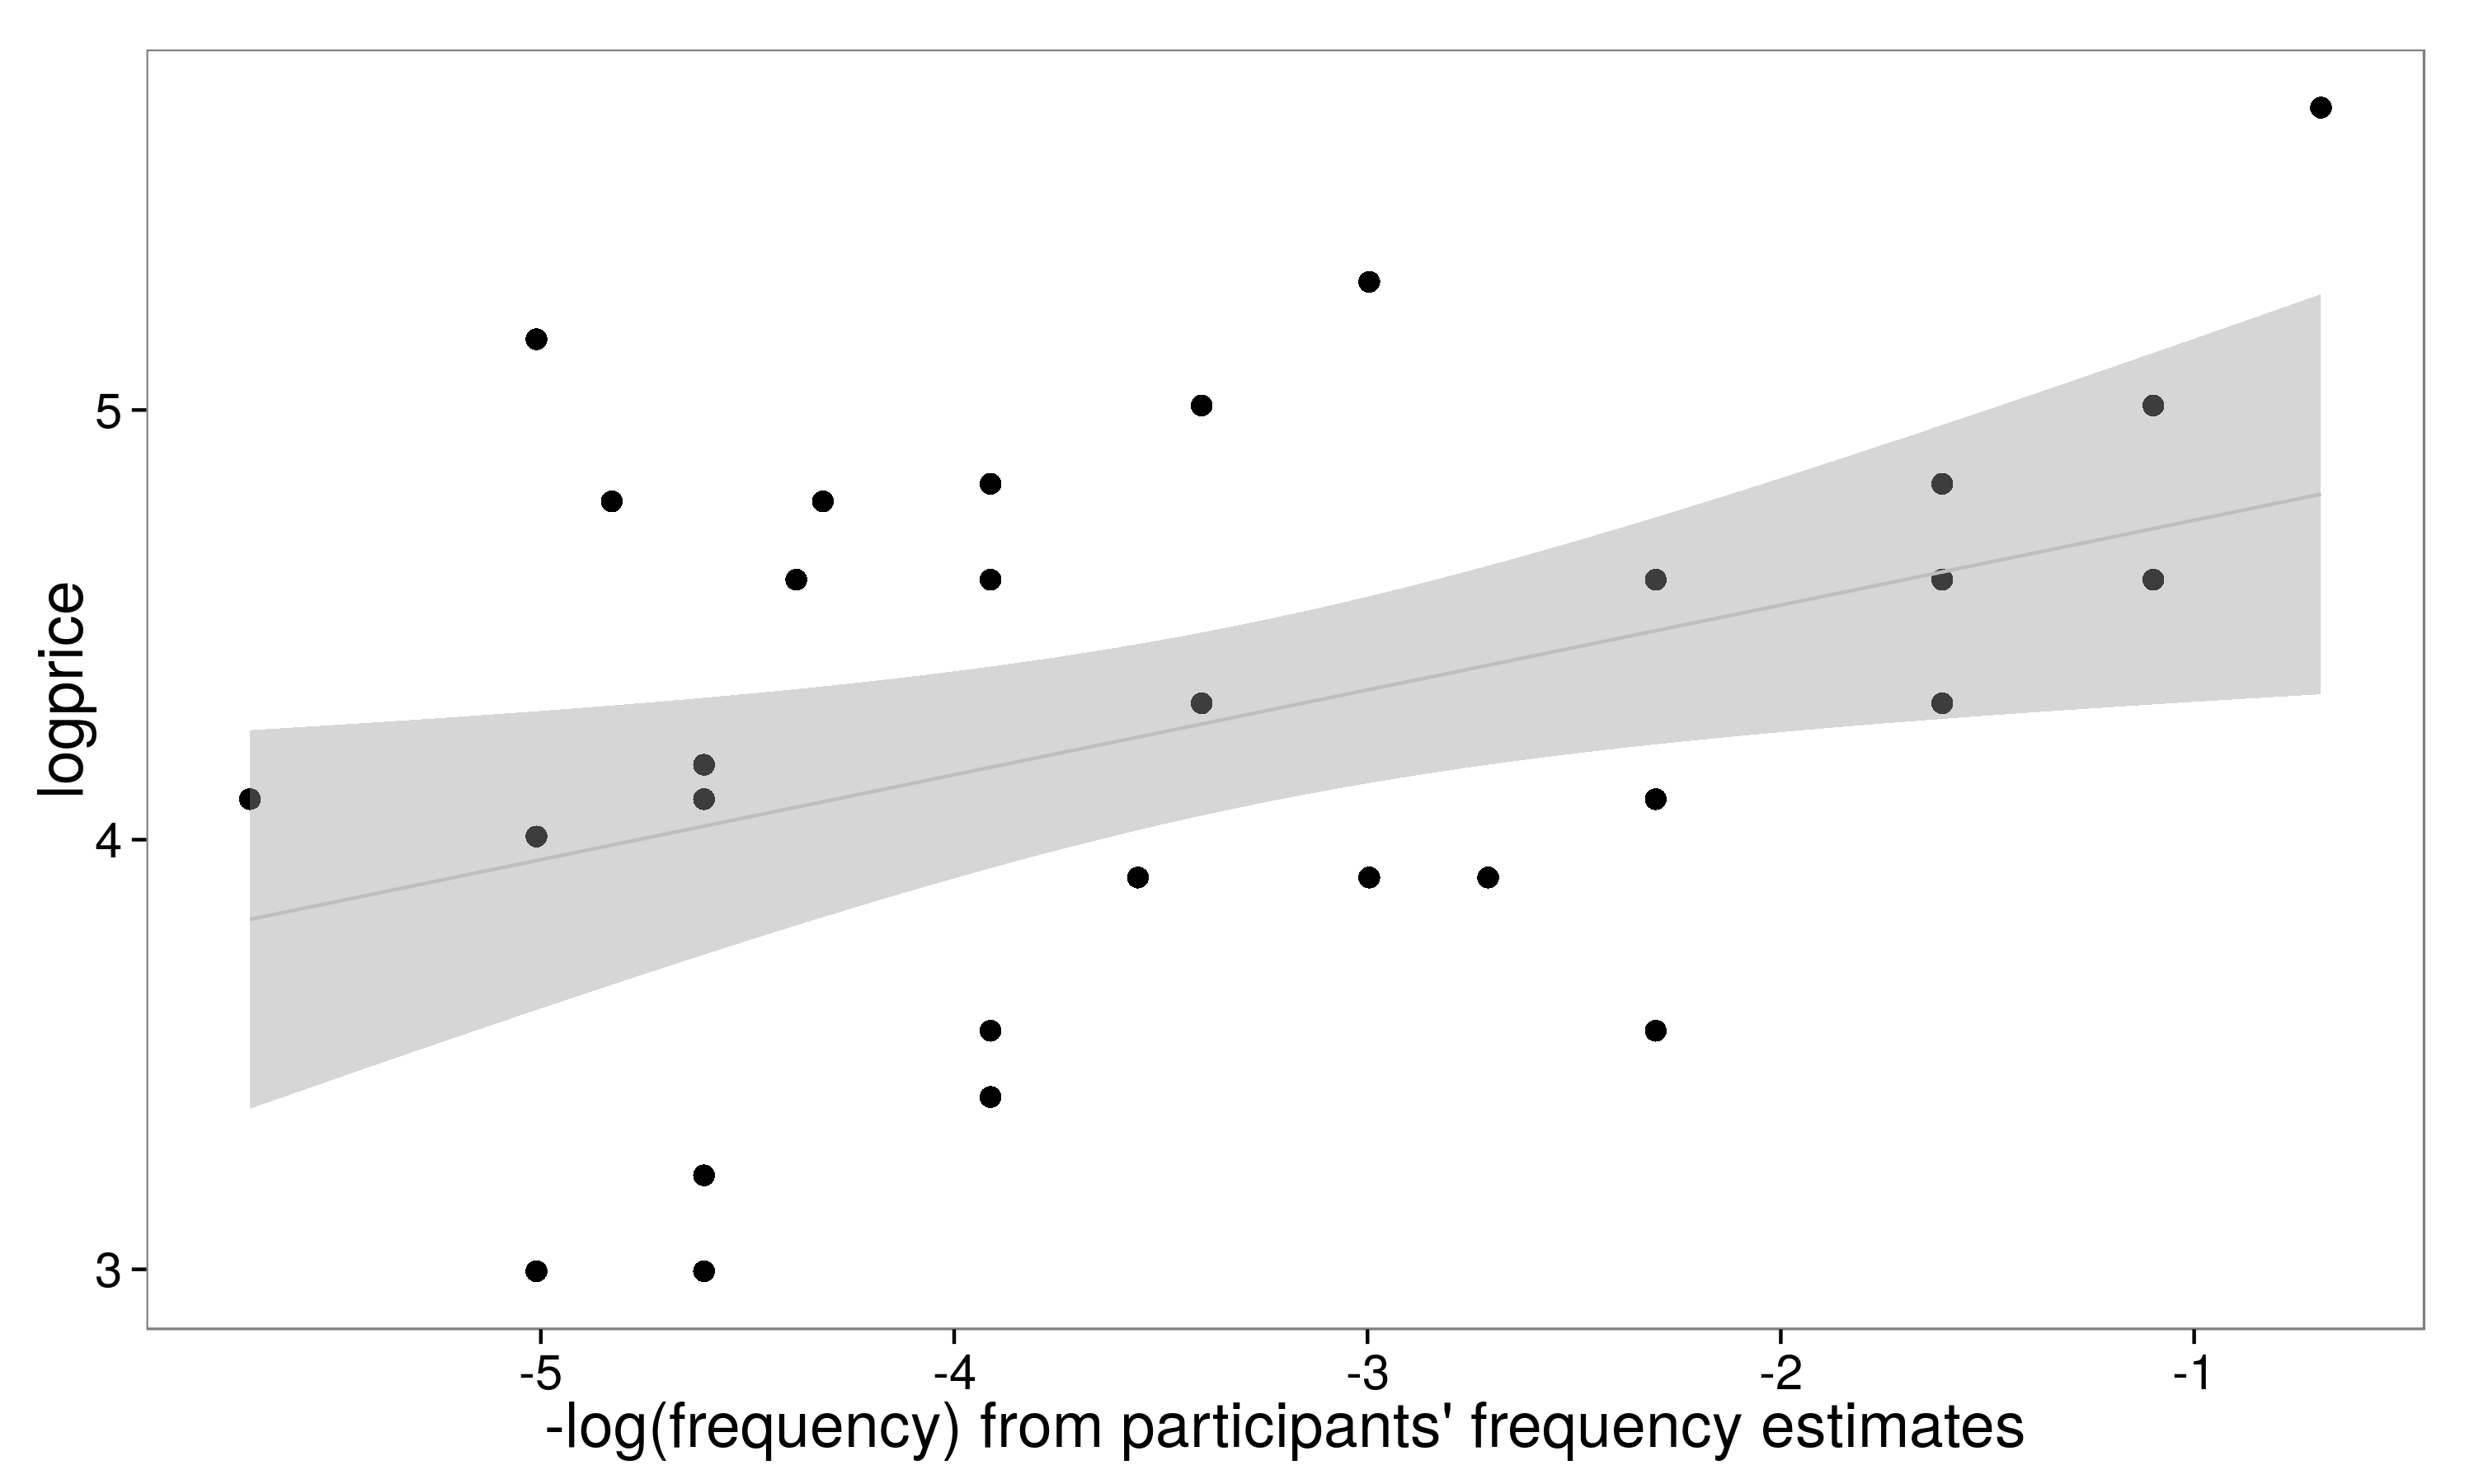
\includegraphics[width=0.48\textwidth]{analysis_files/images/exp3-scatterplot.png}
\end{center}
\caption{Results of Experiment 3. As participants' frequency estimates increase, so do their price estimates.} 
\label{exp3-scatterplot}
\end{figure}

\subsection{Discussion}

\todo[inline]{discussion of experiment3}

\section{Discussion}

\todo[inline]{conclusion}

\section{Acknowledgments}

\nocite{web1t5gram}
\nocite{lewis}

\begin{table}[ht]
 \begin{center}
  \caption{Intensifiers from Experiment 1, number of occurences in Google Web 1T 5grams corpus, and number of syllables.}
  \label{exp1-intensifiers}
  \begin{tabular}{ccc}
   \hline
   ngram & frequency & syllables \\
    \hline
    surpassingly & 11156 & 4 \\
    colossally & 11167 & 4 \\
    terrifically & 62292 & 4 \\
    frightfully & 65389 & 3 \\
    astoundingly & 73041 & 4 \\
    phenomenally & 120769 & 5 \\
    uncommonly & 135747 & 4 \\
    outrageously & 240010 & 4 \\
    fantastically & 250989 & 4 \\
    mightily & 252135 & 3 \\
    supremely & 296134 & 3 \\
    insanely & 359644 & 3 \\
    strikingly & 480417 & 3 \\
    acutely & 493931 & 3 \\
    awfully & 651519 & 3 \\
    decidedly & 817806 & 4 \\
    excessively & 877280 & 4 \\
    extraordinarily & 900456 & 6 \\
    exceedingly & 977435 & 4 \\
    intensely & 1084765 & 3 \\
    markedly & 1213704 & 3 \\
    amazingly & 1384225 & 4 \\
    radically & 1414254 & 3 \\
    unusually & 1583939 & 4 \\
    remarkably & 1902493 & 4 \\
    terribly & 1906059 & 3 \\
    exceptionally & 2054231 & 5 \\
    desperately & 2139968 & 3 \\
    utterly & 2507480 & 3 \\
    notably & 3141835 & 3 \\
    incredibly & 4416030 & 4 \\
    seriously & 12570333 & 4 \\
    truly & 19778608 & 2 \\
    significantly & 19939125 & 5 \\
    totally & 20950052 & 3 \\
    extremely & 21862963 & 3 \\
    particularly & 41066217 & 5 \\
    quite & 55269390 & 1 \\
    especially & 55397873 & 4 \\
    very & 292897993 & 2
  \end{tabular}
 \end{center}
\end{table}


\begin{table}[ht]
\begin{center} 
\caption{Intensifier Lists from Experiment 2: Rankings.} 
\label{exp2-intensifiers} 
\vskip 0.12in
\begin{tabular}{cccc} 
\hline
List A    &  List B & List C & List D \\
\hline
surpassingly & colossally & terrifically & frightfully \\
astoundingly & phenomenally & uncommonly & outrageously \\
fantastically & mightily & supremely & insanely \\
strikingly & acutely & awfully & decidedly \\
excessively & extraordinarily & exceedingly & intensely \\
markedly & amazingly & radically & unusually \\
remarkably & terribly & exceptionally & desperately \\
utterly & notably & incredibly & seriously \\
truly & significantly & totally & extremely \\
particularly & quite & especially & very
\end{tabular}
\end{center}
\end{table}

\bibliographystyle{apacite}

\setlength{\bibleftmargin}{.125in}
\setlength{\bibindent}{-\bibleftmargin}

\bibliography{intensifiers}

\end{document}
